\subsubsection{MSVC}

\RU{Компилируем в}\EN{Compile it in} MSVC 2010:

\lstinputlisting[caption=MSVC 2010: f()]{patterns/12_FPU/1_simple/MSVC_\LANG.asm}

\RU{\FLD берет 8 байт из стека и загружает их в регистр \ST{0}, автоматически конвертируя во внутренний 
80-битный формат (\IT{extended precision}).}
\EN{\FLD takes 8 bytes from stack and load the number into the \ST{0} register, automatically converting 
it into internal 80-bit format \IT{extended precision}).}

\index{x86!\Instructions!FDIV}
\RU{\FDIV делит содержимое регистра \ST{0} на число, лежащее по адресу \TT{\_\_real@40091eb851eb851f} ~--- 
там закодировано значение $3.14$. Синтаксис ассемблера не поддерживает подобные числа, 
так что то что мы там видим, это шестнадцатеричное представление числа \IT{3.14} в формате IEEE 754.}
\EN{\FDIV divides value in the \ST{0} register by number storing at address 
\TT{\_\_real@40091eb851eb851f}~---$3.14$ value is coded there. Assembler syntax missing floating point numbers, so, 
what we see here is hexadecimal representation of \IT{3.14} number in 64-bit IEEE 754 encoded.}

\RU{После выполнения \FDIV, в \ST{0} остается частное\FNQUOTIENT.}
\EN{After \FDIV execution, \ST{0} will hold quotient\FNQUOTIENT.}

\index{x86!\Instructions!FDIVP}
\RU{Кстати, есть еще инструкция \FDIVP, которая делит \ST{1} на \ST{0}, 
выталкивает эти числа из стека и заталкивает результат. 
Если вы знаете язык Forth\FNURLFORTH, то это как раз оно и есть ~--- стековая машина\FNURLSTACK.}
\EN{By the way, there is also \FDIVP instruction, which divides \ST{1} by \ST{0}, 
popping both these values from stack and then pushing result. 
If you know Forth language\FNURLFORTH,
you will quickly understand that this is stack machine\FNURLSTACK.}

\RU{Следующая \FLD заталкивает в стек значение \IT{b}.}
\EN{Next \FLD instruction pushing \IT{b} value into stack.}

\RU{После этого, в \ST{1} перемещается результат деления, а в \ST{0} теперь будет \IT{b}.}
\EN{After that, quotient is placed to the \ST{1} register, and the \ST{0} will hold \IT{b} value.}

\index{x86!\Instructions!FMUL}
\RU{Следующий \FMUL умножает \IT{b} из \ST{0} на значение \TT{\_\_real@4010666666666666} ~--- 
там лежит число 4.1, и оставляет результат в \ST{0}.}
\EN{Next \FMUL instruction do multiplication: \IT{b} from the \ST{0} register by value at 
\TT{\_\_real@4010666666666666} (4.1 number is there) and leaves result in the \ST{0} register.}

\index{x86!\Instructions!FADDP}
\RU{Самая последняя инструкция \FADDP складывает два значения из вершины стека, 
в \ST{1} и затем выталкивает значение, лежащее в \ST{0}, 
таким образом результат сложения остается на вершине стека в \ST{0}.}
\EN{Very last \FADDP instruction adds two values at top of stack, storing result to the \ST{1} 
register and then popping value at \ST{1}, hereby leaving result at top of stack in the \ST{0}.}

\RU{Функция должна вернуть результат в \ST{0}, так что больше ничего здесь не производится, 
кроме эпилога функции.}
\EN{The function must return result in the \ST{0} register, so,
after \FADDP there are no any 
other instructions except of function epilogue.}

\subsubsection{MSVC + \olly}
\index{\olly}

\RU{Я обвел красным в стеке 2 пары 32-битных слов, каждая пара --- 
это double-числа в формате IEEE 754 переданные из \main.}
\EN{I marked by red 2 pairs of 32-bit words in stack. Each pair is double-number in
IEEE 754 format passed from \main.}
\RU{Видно как первая \FLD загружает значение ($1.2$) из стека и помещает в регистр \ST{0}:}
\EN{We see how first \FLD loads a value ($1.2$) from stack and put it into \ST{0} register:}
\figname \ref{fig:FPU_simple_olly_1}.
\RU{Из-за неизбежных ошибок конвертирования числа из 64-битного IEEE 754 в 80-битное (внутреннее в FPU),
мы видим здесь $1.1999...$, что очень близко к $1.2$.}
\EN{Because of unavoidable conversion errors from 64-bit IEEE 754 float point number into 80-bit
(used internally in FPU), we see here $1.999...$, which is close to $1.2$.}
\RU{Прямо сейчас \EIP указывает на следующую инструкцию (\FDIV), загружающую double-число (константу) 
из памяти.}
\EN{\EIP right now is pointing to the next instruction (\FDIV), which loads double-number (a constant)
from memory.}
\RU{Для удобства}\EN{For convenience}, \olly \RU{показывает её значение}\EN{shows its value}: $3.14$.\\
\\
\RU{Трассируем дальше}\EN{Let's trace more}. 
\FDIV \RU{исполнилась}\EN{executed}, \RU{теперь}\EN{now} \ST{0} \RU{содержит}\EN{contain} $0.382...$ 
(\gls{quotient}): \figname \ref{fig:FPU_simple_olly_2}.\\
\\
\RU{Третий шаг}\EN{Third step}: \RU{вторая}\EN{the next} \FLD 
\RU{исполнилась, загружая в \ST{0} $3.4$ (мы видим приближенное число $3.39999...$).}
\EN{executed, loading $3.4$ into \ST{0} (we see here approximated value $3.39999...$).}
\figname \ref{fig:FPU_simple_olly_3}.
\RU{В это время}\EN{At the same time,} \gls{quotient} \IT{\RU{провалилось}\EN{pushed}} 
\RU{в}\EN{into} \ST{1}.
\RU{\EIP в это время указывает не следующую инструкцию}\EN{Right now, \EIP points to the next
instruction}: \FMUL. 
\RU{Она загружает константу}\EN{It loads} $4.1$ \RU{из памяти, так что \olly тоже показывает её здесь}
\EN{constant from memory, so \olly shows it here}.\\
\\
\RU{Затем}\EN{Next}: \FMUL \RU{исполнилась, теперь в \ST{0} произведение}
\EN{was executed, now \gls{product} is in \ST{0}}:
\figname \ref{fig:FPU_simple_olly_4}.\\
\\
\RU{Затем}\EN{Next}: \FADDP \RU{исполнилась, теперь в \ST{0} сумма, а \ST{1} очистился}
\EN{was executed, now result of addition is in \ST{0}, and \ST{1} is cleared}:
\figname \ref{fig:FPU_simple_olly_5}.
\RU{Кстати}\EN{By the way}, \olly, \RU{для краткости}\EN{for brevity}, 
\RU{показывает регистр}\EN{shows the register as} \TT{ST}, \RU{это синоним для}\EN{it's synonymous
for} \ST{0}
\footnote{\RU{Кстати, можно запомнить это как}
\EN{By the way, it could be memorized as} ``Stack Top''.}.

\RU{Сумма остается в \ST{0}, потому что ф-ция возвращает результат своей работы через \ST{0}.}
\EN{Result is leaved in \ST{0}, because the function returns its value in \ST{0}.}
\RU{Позже, \main возьмет это значение оттуда.}
\EN{\main will take this value from the register soon.}\\
\\
\RU{Мы также видим кое-что необычное: значение $13.93...$ теперь находится в \ST{7}.}
\EN{We also see something unusual: $13.93...$ value is now located in \ST{7}.}
\RU{Почему}\EN{Why}?
\RU{Объяснение простое}\EN{It's easy to understand}.
\label{FPU_is_rather_circular_buffer}
\RU{Я писал что регистры в \ac{FPU} представляю собой стек}\EN{As I wrote before, \ac{FPU} registers
is stack}: \ref{FPU_is_stack}. 
\RU{Но это упрощение}\EN{But this is simplification}.
\RU{Представьте, если бы \IT{в железе} было бы так, как описано, тогда при каждом заталкивании 
(или выталкивания) в стек,
все остальные 7 значений нужно было бы передвигать (или копировать) в соседние регистры, 
а это слишком много лишней работы.}
\EN{Just imagine if it would be implemented \IT{in hardware} as it's described, the all 7 register's
contents must be moved (or copied) to adjacent registers, and that's a lot of work.}
\RU{Так что в реальности,
\ac{FPU} имеет просто 8 регистров и указатель (называемый \TT{TOP}), содержащий номер регистра,
которая в текущим момент является ``вершиной стека''.}
\EN{In reality, \ac{FPU} has just 8 registers and a pointer (called \TT{TOP}) which has register number,
which is current ``top of stack''.}
\RU{При заталкивании значения в стек, регистр \TT{TOP} меняется, и указывает на свободный регистр, 
затем значение записывается в этот регистр.}
\EN{When value is pushed into stack, \TT{TOP} register is changing and pointing to a next available register,
and then a value is written to it.}
\RU{При выталкивании значения из стека, процедура обратная, однако, освобожденный регистр не обнуляется}
\EN{The procedure is reversed if value is popped, however, register which was freed is not cleared}
(\RU{наверное, можно было бы сделать, чтобы обнулялся, но это лишняя работа и работало бы медленнее}\EN{it 
could be cleared, but this is another work which may degrade performance}).
\RU{Так что это мы здесь и видим}\EN{So that's what we see here}. 
\RU{Можно сказать что \FADDP сохранила сумму, а затем вытолкнуло один элемент.}
\EN{It can be said, \FADDP saved sum in stack, and then popped one element.}
\RU{Но в реальности, эта инструкция сохранила сумму и затем передвинула регистр \TT{TOP}.}
\EN{But in fact, this instruction saved sum and then shifted \TT{TOP} register.}
\RU{Было бы еще точнее сказать, что регистры \ac{FPU} представляют собой кольцевой буфер.}
\EN{More precisely, \ac{FPU} registers is circular buffer.}

\begin{figure}[H]
\centering
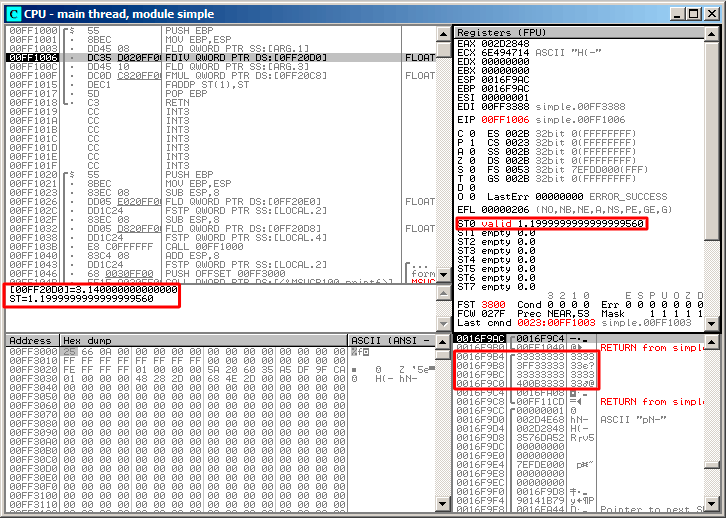
\includegraphics[scale=\FigScale]{patterns/12_FPU/1_simple/olly1.png}
\caption{\olly: \RU{первая \FLD исполнилась}\EN{first \FLD executed}}
\label{fig:FPU_simple_olly_1}
\end{figure}

\begin{figure}[H]
\centering
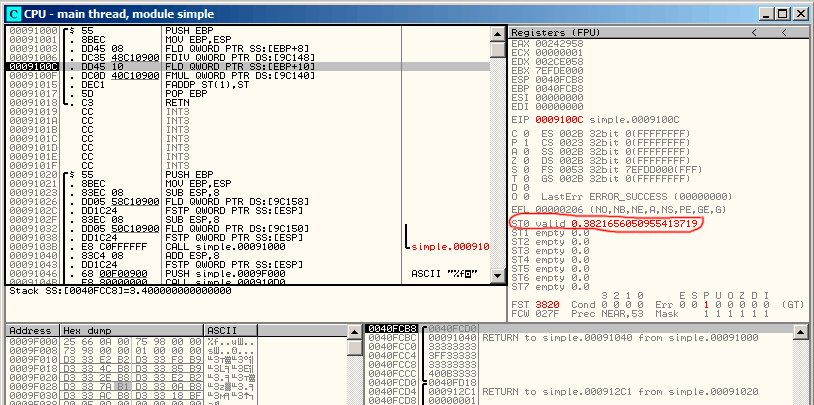
\includegraphics[scale=\FigScale]{patterns/12_FPU/1_simple/olly2.png}
\caption{\olly: \FDIV \RU{исполнилась}\EN{executed}}
\label{fig:FPU_simple_olly_2}
\end{figure}

\begin{figure}[H]
\centering
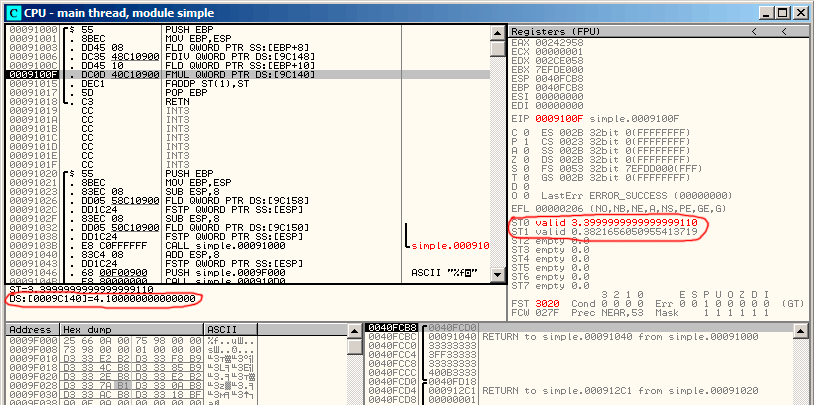
\includegraphics[scale=\FigScale]{patterns/12_FPU/1_simple/olly3.png}
\caption{\olly: \RU{вторая \FLD исполнилась}\EN{second \FLD executed}}
\label{fig:FPU_simple_olly_3}
\end{figure}

\begin{figure}[H]
\centering
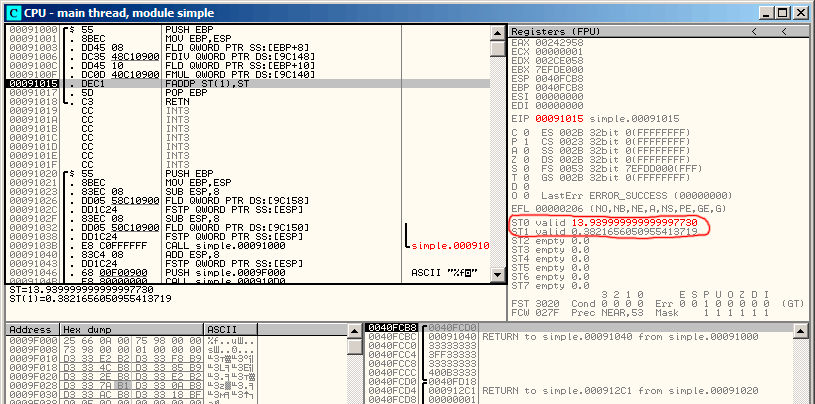
\includegraphics[scale=\FigScale]{patterns/12_FPU/1_simple/olly4.png}
\caption{\olly: \FMUL \RU{исполнилась}\EN{executed}}
\label{fig:FPU_simple_olly_4}
\end{figure}

\begin{figure}[H]
\centering
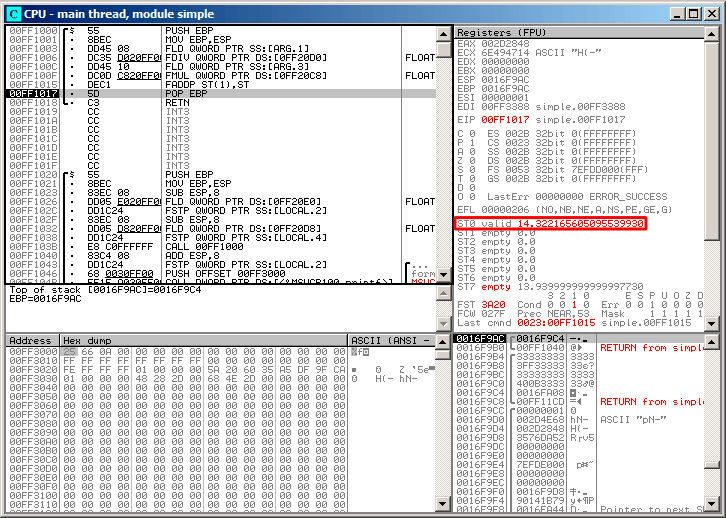
\includegraphics[scale=\FigScale]{patterns/12_FPU/1_simple/olly5.png}
\caption{\olly: \FADDP \RU{исполнилась}\EN{executed}}
\label{fig:FPU_simple_olly_5}
\end{figure}
